\chapter{Scaling rigid-body simulations}
\label{ch:scaling_rigid_body_simulations}

In this final chapter, we provide our most recent results for addressing the problem of generating synthetic data for robot planning and control.
As an initial attempt, in Chapter~\ref{ch:rl_env_for_robotics} we proposed the \scenario \acp{API} and the Gym-Ignition framework that exploited the general purpose simulator Gazebo Sim to sample trajectories for training policies with \ac{RL}.
In Chapter~\ref{ch:learning_from_scratch}, we have validated the framework proposing a scheme that, with experience sampled from Gazebo Sim, was able to train a \ac{RL} policy capable of balancing a humanoid robot by adopting different push-recovery strategies for compensating external disturbances.
We have observed that such a pipeline was characterised by long training times, and identified the simulator as the main bottleneck.

In this chapter, we propose our final simulation architecture for maximising the sampling performance of synthetic data for robot locomotion applications.
Starting from the contact-aware state-space representation proposed in Chapter~\ref{ch:contact_aware_dynamics}, we introduce state-of-the-art \acp{RBDA} for obtaining the terms forming the multibody \acp{EoM} and computing the \emph{forward dynamics} function $\operatorname{FD}(\mathcal{M}, \Qu, \Nu, \Torques, \forcesix_L)$ used in the  $\dot{\mathbf{x}}(t)$ definition of Equation~\ref{equation:tangential_deformation_dynamics} and Equation~\ref{equation:floatig_base_dynamics_with_contacts_state_space}.
Excluding inverse dynamics, that we formulate as the true inverse of the forward dynamics also for floating-base systems, the implementations of the other \acp{RBDA} contain only minor differences compared to the reference formulation presented by \textcite{featherstone_rigid_2008}.
Beyond being denoted with the notation introduced in Chapter~\ref{ch:robot_modelling} that makes explicit the reference frame of quantities like 6D velocities and 6D forces, we provide a unified implementation for both fixed-base and floating-base robots, and our inverse dynamics extends its acceleration to force mapping also to the base link.
In the second part of this chapter, we propose  \jaxsim, a new physics engine in reduced coordinates that, thanks to the implementation of these algorithms in \jax, enables running rigid-body simulations on modern hardware accelerators like \acsp{GPU} and \acsp{TPU}.
In fact, the problem of the previous architectures was not really the general-purpose simulator, but the limited parallel capabilities of \acsp{CPU} in which it was executed.
The \acp{RBDA} presented at the beginning of this chapter enable the combination of model-based algorithms with applications requiring high sampling rates like \acs{RL}.
They have been implemented such that they can be executed transparently on any supported hardware.

\vspace{-3mm}
\section{Floating-base rigid-body dynamics algorithms}
\label{section:fb_rbda}

In previous sections, we described how the dynamics of a floating-base system interacting with a non-flat terrain surface can be described, and how its evolution over time can be obtained through numerical integration.
When we introduced the state-space representations, in Equation~\eqref{equation:floatig_base_dynamics_state_space} and Equation~\eqref{equation:floatig_base_dynamics_with_contacts_state_space}, we used the \emph{forward dynamics} function $\operatorname{FD}(\cdot)$ to describe the dynamics of the floating-base system velocity $\Nu$.
We also mentioned that it can be calculated by inverting the following \ac{EoM}, already defined in Equation~\eqref{eq:eom_multibody_compact}:
%
\begin{equation}
    \label{eq:eom_multibody_compact-rbda}
    M(\Qu) \Nud + h(\Qu, \Nu) = B \Torques + J_\mathcal{L}^\top(\Qu) \forcesix^{ext}_\mathcal{L}
    ,
\end{equation}
%
by assuming the knowledge, at any integration step, of the floating-base version of the mass matrix $M(\Qu)$, the bias-vector $h(\Qu, \Nu)$, and the Jacobians matrix $\jac_\mathcal{L}(\Qu)$.
Calculating the forward dynamics from the \acp{EoM} involves the inversion of the mass matrix that, depending on the number of the number of \acp{DoF}, could be computationally expensive when performed in a simulation loop.
Furthermore, depending on the selected integrator, it might be needed to evaluate the system's dynamics multiple times for each simulation step, computing and inverting $M(\mathbf{q})$ at every evaluation.

Starting from the 80's, efficient iterative algorithms have been proposed to compute the quantities forming Equation~\eqref{eq:eom_multibody_compact-rbda}~\parencite{featherstone_rigid_2008}.
In this section, we provide an adaptation of such algorithms using the notation introduced in Chapter~\ref{ch:robot_modelling}.
We will particularly focus on two operations called \emph{forward dynamics} and \emph{inverse dynamics}, where the latter is the inverse of the former.

\begin{definition*}[Forward Dynamics]
%
Forward dynamics allows to compute the acceleration $\Nud$ of the multibody system $\mathcal{M}$ given the position $\Qu$, the velocity $\Nu$, the generalised input joint forces $\Torques$, and the external link forces $\forcesix^{ext}_\mathcal{L}$.
It can be described with the following function:
%
\begin{equation*}
    \dot{\boldsymbol{\nu}} = \operatorname{FD}(\mathcal{M}, \mathbf{q}, \boldsymbol{\nu}, \boldsymbol{\tau}, \forcesix^{ext}_\mathcal{L})
    .
\end{equation*}
%
\end{definition*}

\begin{definition*}[Inverse Dynamics]
\label{def:id}
%
Inverse dynamics allows to compute the joint torques $\Torques$ to apply on the multibody system $\mathcal{M}$ to produce a desired acceleration $\Nud$ starting from the system's position $\Qu$ and velocity $\Nu$ together with the link external forces $\forcesix^{ext}_\mathcal{L}$.
It also calculates the 6D force $\forcesix[W]_{B}$ that, when applied to the base link, explains the component of the base acceleration $\accsix[W]_{W,B}$ part of $\Nud$ that is not due gravitational effects nor external forces.
It can be described with the following function:
%
\begin{equation*}
    (\forcesix[W]_{B}, \Torques) = \operatorname{ID}(\mathcal{M}, \Qu, \Nu, \Nud, \forcesix^{ext}_\mathcal{L})
    .
\end{equation*}
%
\end{definition*}

Beyond contact-related functionality, forward dynamics is the only necessary function for implementing a rigid-body simulator in reduced coordinates.
However, we will see that inverse dynamics is necessary to compute all the terms forming the multibody \acp{EoM}~\eqref{eq:eom_multibody_compact-rbda}.
In fact, the most straightforward implementation of forward dynamics involves isolating $\Nud$ from Equation~\eqref{eq:eom_multibody_compact}.
This computation, however, can be optimised by exploiting the sparsity of the kinematic tree that describes the multibody system.
We will also present an algorithm that can efficiently compute forward dynamics by exploiting an iterative approach.

\subsection{Implementation differences}

The algorithms introduced in the next sections are an adaptation of those presented by \textcite{featherstone_rigid_2008}.
Compared to the reference algorithms, our implementation contains the following modifications:
%
\begin{enumerate}
%
\item We present unified algorithms that work on both fixed-base and floating-base models.
We allow specifying a custom pose of fixed-base models, and assume their base velocity and acceleration to be zero.
%
\item We use the notation of 6D quantities introduced in Chapter~\ref{ch:robot_modelling} that makes explicit the reference frame of 6D quantities like velocities, accelerations, and forces.
%
\item All the input and output quantities are expressed in inertial representation, with the exclusion of the mass matrix $M(\Qu)$ and the Jacobian $\jac_\mathcal{L}(\Qu)$ that are computed for efficiency reasons in body-fixed representation.
Section~\ref{sec:change_of_base_variables} provides the transformations to apply for changing the velocity representation of the computed quantities.
%
\item We assume the model $\mathcal{M}$ only containing joints with 1 \ac{DoF}.
As a consequence, all joint quantities $\Shape, \Shaped, \Shapedd, \Torques \in \realn^n$, where $n = N_B - 1$.
%
\item If the model description contains fixed joints, we assume they can be removed from the kinematic tree through a \emph{lumping} process.
If links $P$ and $C$ are connected with a fixed joint, the lumping process replaces the link pair $(P, C)$ with an equivalent link $\tilde{P}$ associated to the frame of $P$, having an equivalent 6D inertia $\masssix[\tilde{P}]_{\tilde{P}} = \masssix[P]_P + \transfor[P]^C \masssix[C]_C \transvel[C]_P$.
%
\item The floating-base \ac{RNEA} implemented in \textcite[Section 9.5]{featherstone_rigid_2008} is not a proper $\operatorname{ID}$ function as it was defined in Definition~\ref{def:id}, since it treats the base acceleration as an output instead of being an input.
In other words, the reference $\operatorname{FD}$ and $\operatorname{ID}$ are not inverse functions.
In fact, the reference implementation is presented as a hybrid-dynamics problem, where the base acceleration is computed through a forward pass.
Our \acs{RNEA} implementation instead accepts as additional input the acceleration of the base $\accsix[W]_{W,B}$, that forms the first six elements of the generalized acceleration $\Nud[W]$.
We assume this acceleration being provided externally, either measured or estimated if applied on real robots.
Our algorithm returns the 6D force $\forcesix[W]_B$ that, when exerted on the base link together with the optional external forces, produces the provided base acceleration.
The effects of gravity are handled internally.
%
\end{enumerate}

\subsection{Model specification}

The information about the kinematics, the inertial properties of all links, and the joint types, are included in the model specification $\mathcal{M}$\footnote{All information included in the model $\mathcal{M}$ could be directly computed from model descriptions like \acs{SDF}, \acs{URDF}, \acs{MJCF}, \etc}:
%
\begin{enumerate}
%
\item The numbering of the links follows the scheme introduced in Section~\ref{sec:multibody_topology}, starting from the index 0 assigned to the base link.
The base link $B$ is selected when parsing the model description, and it is the root of the kinematic tree.
$N_B$ is the total number of bodies belonging to $\mathcal{M}$.
When applied to fixed-base models, the algorithms ignore their base link dynamics.
%
\item The parent-to-child transforms $\homo[\lambda(i)]_i$ for all links $L \in \{\mathcal{L}/B\}$.
We denote the link frames with the link index, \ie $\homo[0]_1$ denotes the transform between link $0$ and link $1$.
%
\item The \emph{parent array} $\lambda(i)$ that, given a link with index $i$, returns the index of its parent link.
%
\item The array $\kappa(i)$ that, given a link $L$ with index $i$, returns the joints connecting all links of the path $\pi_B(L)$.
%
\item The 6D inertia of all links $\masssix_L$, expressed in link frame.
%
\item For each joint $i$, connecting the link pair $(\lambda(i), i)$, $\mathcal{M}$ includes the velocity transformation $\transvel[\operatorname{pre}(i)]_{\lambda(i)}$ that locates the predecessor frame $\operatorname{pre}(i)$ of joint $i$ from the frame $\lambda(i)$ of its parent link (refer to Figure~\ref{fig:joint_model} for a visual feedback).
%
\item The type of all joints, retrieved through the $\text{\spacedlowsmallcaps{Jtype}}(\cdot)$ function from the joint index.
%
\item A function $\text{\spacedlowsmallcaps{Jcalc}}(\cdot)$ accepting a joint type and a joint position $\shape \in \realn$ that returns the motion subspace $\subspace$ and the joint velocity transform $\transvel[\operatorname{suc}(\cdot)]_{\operatorname{pre}(\cdot)}$ corresponding to the given joint position (refer to Figure~\ref{fig:joint_model} for a visual feedback).
%
\end{enumerate}
%
It is worth noting that all these quantities are constant, therefore $\mathcal{M}$ is immutable.
In the algorithm listings, we use a superscript $(\cdot)^\mathcal{M}$ to mark these constant model quantities.

\subsection{Remarks}
%
In the algorithm listings of the next sections, we use the following notation and assumptions:
%
\begin{enumerate}
%
\item The relation between the transformation of 6D forces and 6D velocities is $\transfor[A]^B = \transvel[B]_A^\top$.
When needed, we often exploit the relation $\transfor[\lambda(i)]^i = \transvel[i]_{\lambda(i)}^\top$.
%
\item If $g \in \realn^+$ is the gravitational acceleration, we denote the corresponding 6D acceleration as $\accsix[W]_g = (0; 0; -g; \zeros_3) \in \realn^6$.
%
\item Kinematic and dynamic quantities are propagated between links connected with joints with the relations introduced in Section~\ref{sec:joint_kin_dyn_propagation}.
Regarding joint accelerations, we assume the presence of joints with only 1~\ac{DoF} and a constant motion subspace, resulting to Equation~\eqref{eq:joint_model_acceleration_propagation} and the considerations reported in Definition~\ref{definition:propagation_accelerations}.
%
\item We use 1-based indexing for vectors and matrices.
This means that, if $A \in \realn^{n \times m}$, the top-left element is $A_{(1, 1)}$ and the bottom-right $A_{(n,m)}$.
Selectors of multiple elements use the $:$ delimiter, for example $A_{(1:3,1:3)}$ is the top-left $3 \times 3$ block, and $A_{(1:3,1)}$ its first column.
Note that, while this notation simplifies pseudocode, it requires a careful implementation with 0-based array libraries.
%
\end{enumerate}

\subsection{CRBA: Composite Rigid Body Algorithm}

The \ac{CRBA} is an efficient algorithm that computes the body-fixed mass matrix $M_B(\Shape)$ defined in Equation~\eqref{eq:mass_matrix} having the following structure, already discussed in Remark~\ref{remark:mass_matrix_structure}:
%
\begin{equation*}
    M_B(\Shape) = 
    \begin{bmatrix}
        \masssix[B](\Shape) & F(\Shape) \\
        F^\top(\Shape) & H(\Shape)
    \end{bmatrix}
    \in \realn^{(6+n)\times(6+n)}
    .
\end{equation*}

A reference of the \ac{CRBA} for fixed-base and floating-base systems can be found in \parencite[Section~6.2 and Section~9.4]{featherstone_rigid_2008}.
Algorithm~\ref{algo:crba} reports a unified version of the \ac{CRBA} for both floating-base and fixed-base systems.
It calculates the body-fixed mass matrix $M_B(\Shape)$, that in this representation only depends on the shape $\Shape$.
The knowledge of the mass matrix is the first element that allows the calculation of the forward dynamics from the system's \acp{EoM}.
The algorithm takes the following inputs:
%
\begin{itemize}
    \item $\mathcal{M}$: the model containing the multibody system constant data;
    \item $\Shape \in \realn^n$: the joint positions of all joints belonging to the multibody system;
\end{itemize}
%
and provides the following output:
%
\begin{itemize}
    \item $M \in \realn^{(6+n)\times(6+n)}$: the floating-base mass matrix in body-fixed velocity representation.
\end{itemize}
%
The resulting mass matrix can be converted to other velocity representations with the change of coordinates introduced in Section~\ref{sec:change_of_base_variables}.

\begin{algorithm}
\caption{Composite Rigid Body Algorithm}
\label{algo:crba}
\begin{algorithmic}[1]
\small

\State \textbf{inputs} $(\mathcal{M}, \Shape)$

\State $\masssix^c_0 = \masssix_0^{\mathcal{M}}$
\State $\transvel[0]_0 = \eye_6$

\For{$i = 1 \textbf{ to } N_B^{\mathcal{M}}$}
    \Comment{Propagate kinematics}
    \State $[\transvel[i]_{pre}, \mathbf{S}_i] = \Call{jcalc}{\Call{jtype}{i}, s_i}$
    \State $\transvel[i]_{\lambda(i)} = \transvel[i]_{pre} \transvel[pre]_{\lambda(i)}^{\mathcal{M}}$
    \State $\transvel[i]_{0} = \transvel[i]_{\lambda(i)} \transvel[\lambda(i)]_0$

    \State $\masssix^c_i = \masssix_i^{\mathcal{M}}$
    \Comment{Initialize composite inertia}
\EndFor

\State $M = \boldsymbol{0}_{(6+n)\times(6+n)}$

\For{$i = N_B^{\mathcal{M}} \textbf{ to } 1$}
    \State $\masssix^c_{\lambda(i)} = \masssix^c_{\lambda(i)} + \transvel[i]_{\lambda(i)}^\top \masssix^c_i \transvel[i]_{\lambda(i)}$
    
    \LComment{Compute $M_{jj}$}
    \State $\mathbf{F}_i = \masssix^c_i \mathbf{S}_i$
    \State $M_{(i+6,i+6)} = \mathbf{S}_i^\top \mathbf{F}_i$
    \State $j = i$
    \While{$\lambda(j) \neq 0$}
        \State $\mathbf{F}_i = \transvel[j]_{\lambda(j)}^\top \mathbf{F}_i$
        \State $j = \lambda(j)$
        \State $M_{(i+6,j+6)} = \mathbf{F}^\top_i \mathbf{S}_j$
        \State $M_{(j+6,i+6)} = M_{(i+6,j+6)}$
    \EndWhile

    \LComment{Compute $M_{jb}$ and $M_{bj}$}
    \State $\mathbf{F}_i = \transvel[j]_0^\top \mathbf{F}_i$
    \State $M_{(i+6, 1:6)} = \mathbf{F}_i^\top$
    \State $M_{(1:6, i+6)} = \mathbf{F}_i$
\EndFor

\State $M_{(1:6, 1:6)} = \masssix^c_0$
\Comment{Compute $M_{bb}$}

\State \textbf{output} $M$

\end{algorithmic}
\end{algorithm}

\subsection{RNEA: Recursive Newton-Euler Algorithm}

The \ac{RNEA} is an efficient algorithm that computes the inverse dynamics of a multibody system:
%
\begin{equation*}
    \boldsymbol{\tau} = \operatorname{ID}(\mathcal{M}, \mathbf{q}, \boldsymbol{\nu}, \dot{\boldsymbol{\nu}}, \forcesix^{ext}_\mathcal{L})
    .
\end{equation*}
%
A reference of the \ac{RNEA} for fixed-base and floating base systems can be found in \parencite[Section~5.3 and Section~9.5]{featherstone_rigid_2008}.
Algorithm~\ref{algo:rnea} reports a unified version of the \ac{RNEA} for both floating-base and fixed-base systems.
It calculates the joint torques to be applied to the multibody system to produce the provided acceleration starting from a given position and velocity.
In particular, it takes the following inputs:
%
\begin{itemize}
    \item $\mathcal{M}$: the model containing the multibody system constant data;
    \item $\Shape, \Shaped, \Shapedd \in \realn^n$: the positions, velocities, and accelerations of all joints belonging to the multibody system;
    \item $\transvel[W]_B \in \realn^{6\times6}$: the velocity transform from the base link $B$ to the world link $W$;
    \item $\velsix[W]_{W,B} \in \realn^6$: the inertial-fixed velocity of the base link $B$;
    \item $\accsix[W]_{W,B} \in \realn^6$: the 6D inertial-fixed intrinsic acceleration of the base link $B$ that, considering the reference frame, corresponds to the apparent acceleration $\accsix[W]_{W,B} = {}^W \dot{\mathbf{v}}_{W,B}$ ;
    \item $\forcesix[W]^{ext}_\mathcal{L} \in \realn^{N_B^\mathcal{M} \times 6}$: the matrix stacking, for all $N_B^\mathcal{M}$ links belonging to the model, their corresponding external force $\forcesix[W]_i^{ext} \in \realn^6$ is expressed in world coordinates;
    \item $\accsix[W]_g \in \realn^6$: the gravitational 6D acceleration;
\end{itemize}
%
and provides the following outputs:
%
\begin{itemize}
    \item $\Torques \in \realn^n$: the generalized forces of all joints belonging to the multibody system;
    \item $\forcesix_0 \in \realn^6$: if the model is floating base, the 6D force $\forcesix[W]_B$ that, applied to the base link, produces the real acceleration $\accsix[W]_{W,B}$ provided as input, or zero if fixed-base.
\end{itemize}

\ac{RNEA} can also be used to efficiently compute other components of the \ac{EoM} necessary to compute the forward dynamics.
In fact, the following relations hold:
%
\begin{equation*}
    \begin{cases}
        g(\Qu) = \operatorname{ID}(\mathcal{M}, \Qu, \zeros_{6+n}, \zeros_{6+n}, \zeros_{6 n_L}) \\
        h(\Qu, \Nu) = \operatorname{ID}(\mathcal{M}, \Qu, \Nu, \zeros_{6+n}, \zeros_{6 n_L}) \\
        C(\Qu, \Nu) \Nu = h(\Qu, \Nu) - g(\Qu)
\end{cases}
.
\end{equation*}
%
This implementation provides such quantities in inertial-fixed representation, and can be converted to the other ones using the change of coordinates provided in Section~\ref{sec:change_of_base_variables}.

\begin{algorithm}
\caption{Recursive Newton-Euler Algorithm}
\label{algo:rnea}

\begin{algorithmic}[1]
\small

\State \textbf{inputs} $\left(\mathcal{M}, \Shape, \Shaped, \Shapedd, \transvel[W]_B, \velsix[W]_{W,B}, \accsix[W]_{W,B}, \forcesix[W]^{ext}_\mathcal{L}, \accsix[W]_g \right)$

\State $\transvel[0]_{W} = \transvel[B]_W$
\Comment{Initialise base transform}
\State $\transvel[0]_{0} = \eye_6$
\State $\forcesix_0 = \zeros_6$

\If{floating}
    \Comment{Initialise base quantities}
    \State $\transfor[0]^W = \transvel[0]_W^{-\top}$
    \State $\velsix_0 = \velsix[0]_{W,0} = \transvel[0]_{W} \velsix[W]_{W,0}$
    \State $\accsixproper_0 = \accsixproper[0]_{W,0} = \transvel[0]_{W} (\accsix[W]_{W,B} - \accsix[W]_g)$
    \State $\forcesix_0 = \forcesix[B]_B = \masssix_0^{\mathcal{M}} \accsixproper_0 + \crossforsix[\velsix_0] \masssix_0^{\mathcal{M}} \velsix_0 - \transfor[0]^W \forcesix[W]_0^{ext}$
\EndIf

\For{$i = 1 \textbf{ to } N_B^{\mathcal{M}}$}
    \Comment{Forward pass}
        
    \LComment{Compute parent-to-child transform}
    \State $[\transvel[i]_{pre}, \mathbf{S}_i] = \Call{jcalc}{\Call{jtype}{i}, s_i}$
    \State $\transvel[i]_{\lambda(i)} = \transvel[i]_{pre} \transvel[pre]_{\lambda(i)}^{\mathcal{M}}$
    
    \LComment{Propagate link velocity and acceleration}
    \State $\velsix_i = \velsix[i]_{\lambda(i),i} = \transvel[i]_{\lambda(i)} \velsix_{\lambda(i)} + \mathbf{S}_i \dot{s}_i$
    \State $\accsixproper_i = \accsixproper[i]_{\lambda(i),i} = \transvel[i]_{\lambda(i)} \accsixproper_{\lambda(i)} + \mathbf{S}_i \ddot{s}_i + \crossvelsix[\velsix_i] \mathbf{S}_i \dot{s}_i$
    
    \LComment{Start propagating link force}
    \State $\transvel[i]_0 = \transvel[i]_{\lambda(i)} \transvel[\lambda(i)]_0$
    \State $\transfor[i]^W = (\transvel[i]_0 \transvel[0]_W)^{-\top}$
    \State $\forcesix_i = \forcesix[i]_i = \masssix_i^{\mathcal{M}} \accsixproper_i + \crossforsix[\velsix_i] \masssix_i^{\mathcal{M}} \velsix_i - \transfor[i]^W \forcesix[W]_i^{ext}$
\EndFor

\For{$i = N_B^{\mathcal{M}} \textbf{ to } 1$}
    \Comment{Backward pass}
    \State $\tau_i = \mathbf{S}_i^\top \forcesix_i$
    \If{$\lambda(i) \neq 0$ or floating}
        \Comment{Finalize link force propagation}
        \State $\forcesix_{\lambda(i)} = \forcesix_{\lambda(i)} + \transvel[i]_{\lambda(i)}^\top \forcesix_i$
    \EndIf
\EndFor

\State \textbf{outputs} $\left( \Torques, \forcesix_0 \right)$
%
\end{algorithmic}
\end{algorithm}

\subsection{Free-floating Jacobian}

The free-floating Jacobian of a link $E \in \mathcal{L}$, already defined in Definition~\ref{definition:link_jacobian} has the following block structure:
%
\begin{equation*}
    \jac[Y]_{W,E/X}(\Qu) =
        \begin{bmatrix}
            \transvel[Y]_X & {}^Y S_{B,E}(\Shape)
        \end{bmatrix}
        .
\end{equation*}
%
The relevant equations to compute the Jacobian matrix for fixed-base and floating-base systems can be found in \parencite[Section~4.1 and Section~9.5]{featherstone_rigid_2008}.
Algorithm~\ref{algo:jacobian} reports a unified version for the computation of the left-trivialized floating-base Jacobian for left-trivialized system velocities $\jac[E]_{W,E/B}$.
The following relation provides the intended usage that highlights the correct representations:
%
\begin{equation*}
    \velsix[E]_{W,E} = \jac[E]_{W,E/B}(\Qu) \Nu[B]
    .
\end{equation*}
%
Note that using these representations for input and output velocities, the free-floating Jacobian does not depend on base variables.
The algorithm takes the following inputs:
%
\begin{itemize}
    \item $\mathcal{M}$: the model containing the multibody system constant data;
    \item $\Shape \in \realn^n$: the joint positions of all joints belonging to the multibody system;
    \item $\operatorname{idx}(L_i) \in 0 \cup \mathbb{N}$: the index of the link of the returned Jacobian;
\end{itemize}
%
and returns the following output:
%
\begin{itemize}
    \item $\jac \in \realn^{6\times n}$: the free-floating Jacobian of the link $L_i$.
\end{itemize}

\begin{algorithm}
\caption{Floating-base doubly-left Jacobian}
\label{algo:jacobian}
\begin{algorithmic}[1]
\small

\State \textbf{inputs} $\left(\mathcal{M}, \Shape, L_i\right)$

\State $\transvel[0]_0 = \eye_6$

\For{$i = 1 \textbf{ to } N_B^{\mathcal{M}}$}
    \Comment{Propagate kinematics}

    \State $[\transvel[i]_{pre}, \mathbf{S}_i] = \Call{jcalc}{\Call{jtype}{i}, s_i}$
    \State $\transvel[i]_{\lambda(i)} = \transvel[i]_{pre} \transvel[pre]_{\lambda(i)}^{\mathcal{M}}$
    \State $\transvel[i]_0 = \transvel[i]_{\lambda(i)} \transvel[\lambda(i)]_0$

\EndFor

\State $J = \zeros_{6 \times (6+N_B^{\mathcal{M}})}$

\State $J_{(1:6, 1:6)} = \transvel[L_i]_0$
\Comment{Compute $J_b$}

\For{$i = 1 \textbf{ to } N_B^{\mathcal{M}}$}
    \Comment{Compute $J_s$}
    \If{$i \in \kappa^{\mathcal{M}}(L_i)$}
        \State $J_{(1:6, 6+i)} = \transvel[L_i]_0 \transvel[0]_i \mathbf{S}_i$
    \EndIf
\EndFor

\State \textbf{output} $J$

\end{algorithmic}
\end{algorithm}

\subsection{ABA: Articulated-Body Algorithm}

Given a model $\mathcal{M}$, the forward dynamics computation is defined with the following signature:
%
\begin{equation*}
    \dot{\boldsymbol{\nu}} = \operatorname{FD}(\mathcal{M}, \mathbf{q}, \boldsymbol{\nu}, \boldsymbol{\tau}, \forcesix^{ext}_\mathcal{L})
    .
\end{equation*}
%
As we already mentioned earlier in this chapter, forward dynamics can be computed by inverting the \ac{EoM}:
%
\begin{equation*}
    \Nud =
    \begin{bmatrix}
        \accsix_{W,B} \\ \Shapedd
    \end{bmatrix} =
    M^{-1}(\Qu) \left[ B \Torques - h(\Qu, \Nu) + \jac_\mathcal{L}^\top(\Qu) \forcesix^{ext}_\mathcal{L} \right]
    .
\end{equation*}
%
The previous algorithms provide all the necessary components for this computation.

The computation and inversion of $M$, depending on the number of the system's \acp{DoF}, could be expensive.
The \ac{ABA} is an efficient iterative algorithm to compute the forward dynamics.
A reference for fixed-base and floating-base systems can be found in \parencite[Section~7.3 and Section~9.4]{featherstone_rigid_2008}.
Algorithm~\ref{algo:aba} reports a unified version of \ac{ABA} for both floating-base and fixed-based systems.
It takes the following inputs:
%
\begin{itemize}
    \item $\mathcal{M}$: the model containing the multibody system constant data;
    \item $\Shape, \Shaped \in \realn^n$: the positions and velocities of all joints belonging to the multibody system;
    \item $\Torques \in \realn^n$: the generalised forces of all joints belonging to the multibody system;
    \item $\transvel[W]_B \in \realn^{6\times6}$: the velocity transform from the base link $B$ to the world link $W$;
    \item $\velsix[W]_{W,B} \in \realn^6$: the inertial-fixed velocity of the base link $B$;
    \item $\forcesix[W]^{ext}_\mathcal{L} \in \realn^{N_B^\mathcal{M} \times 6}$: the matrix stacking, for all $N_B^\mathcal{M}$ links belonging to the model, their corresponding external force $\forcesix[W]_i^{ext} \in \realn^6$ is expressed in world coordinates;
    \item $\accsix[W]_g \in \realn^6$: the gravitational 6D acceleration;
\end{itemize}
%
and provides the following outputs:
%
\begin{itemize}
    \item $\Shapedd \in \realn^n$: the accelerations of all joints belonging to the multibody system;
    \item $\accsix[W]_{W,B} \in \realn^6$: if the model is floating base, the 6D inertial-fixed intrinsic acceleration of the base link $B$ that, considering the reference frame, corresponds to the apparent acceleration $\accsix[W]_{W,B} = {}^W \dot{\mathbf{v}}_{W,B}$.
\end{itemize}

For simulation purposes, forward dynamics is the only necessary function to implement, and \ac{ABA} provides an efficient option.
Considering the state-space system introduced in Equation~\eqref{equation:floatig_base_dynamics_state_space}, we can now define the state variables $\mathbf{x}$ and it derivative $\dot{\mathbf{x}}$ as:
%
\begin{equation*}
    \mathbf{x}(t) =
    \begin{bmatrix} \Qu \\ \Nu \end{bmatrix} =
    \begin{bmatrix}
        \begin{pmatrix}
            \pos[W]_B \\
            \quat[W]_B \\
            \Shape
        \end{pmatrix}
        \\
        \begin{pmatrix}
            \vellin[W]_{W,B} \\
            \velang[W]_{W,B} \\
            \Shaped
        \end{pmatrix}
    \end{bmatrix}
    ,
\end{equation*}
%
\begin{align*}
    \dot{\mathbf{x}}(t) =
    \begin{bmatrix}
        \dot{\mathbf{q}} \\ \dot{\boldsymbol{\nu}}
    \end{bmatrix} =
    \begin{bmatrix}
        \begin{pmatrix}
            \vellin[{B[W]}]_{W,B} \\
            \frac{1}{2} \operatorname{S}\left( \rot[B]_W \velang[W]_{W,B} \right) \quat[W]_B \\
            \dot{\mathbf{s}}
        \end{pmatrix}
        \\
        \begin{pmatrix}
            \accsix[W]_{W,B} \\
            \Shapedd
        \end{pmatrix}
    \end{bmatrix}
    .
\end{align*}

\begin{algorithm}
\caption{Articulated Body Algorithm}

\label{algo:aba}

\begin{algorithmic}[1]

\setstretch{1.2}
\small

\State \textbf{inputs} $\left(\mathcal{M}, \Shape, \Shaped, \Torques, \transvel[W]_B, \velsix[W]_{W,B}, \forcesix[W]^{ext}_\mathcal{L}, \accsix[W]_g \right)$

\State $\transvel[0]_{W} = \transvel[B]_W$
\Comment{Initialise base transform}
\State $\transvel[0]_{0} = \eye_6$

% \LComment{Initialize base state}
\If{floating}
    \Comment{Initialise base quantities}
    \State $\transfor[0]^W = \transvel[0]_W^{-\top}$
    \State $\velsix_0 = \velsix[0]_{W,0} = \transvel[0]_{W} \velsix[W]_{W,0}$
    \State $\masssix^A_0 = \masssix_0^{\mathcal{M}}$
    \State $\mathbf{p}^A_0 = \crossforsix[\velsix_0] \masssix_0^A \velsix_0 - \transfor[0]^W \forcesix[W]_0^{ext}$
\EndIf

\For{$i = 1 \textbf{ to } N_B^{\mathcal{M}}$}
    \Comment{Pass 1}
    
    \LComment{Compute parent-to-child transform}
    \State $[\transvel[i]_{pre}, \mathbf{S}_i] = \Call{jcalc}{\Call{jtype}{i}, s_i}$
    \State $\transvel[i]_{\lambda(i)} = \transvel[i]_{pre} \transvel[pre]_{\lambda(i)}^{\mathcal{M}}$
    
    \LComment{Propagate link velocity}
    \State $\velsix_J = \mathbf{S}_i \dot{s}_i$
    \State $\velsix_i = \velsix[i]_{\lambda(i),i} = \transvel[i]_{\lambda(i)} \velsix_{\lambda(i)} + \velsix_J$
    \State $\mathbf{c}_i = \crossvelsix[\velsix_i] \velsix_J$
    
    \State $\masssix^A_i = \masssix_i^{\mathcal{M}}$
    \Comment{Initialise articulated-body inertia}
    
    \LComment{Initialise articulated-body bias forces}
    \State $\transvel[i]_0 = \transvel[i]_{\lambda(i)} \transvel[\lambda(i)]_0$
    \State $\transfor[i]^W = (\transvel[i]_0 \transvel[0]_W)^{-\top}$
    \State $\mathbf{p}^A_i = \crossforsix[\velsix_i] \masssix_i \velsix_i - \transfor[i]^W \forcesix[W]_i^{ext}$

\EndFor

\For{$i = N_B^{\mathcal{M}} \textbf{ to } 1$}
    \Comment{Pass 2}
    
    \LComment{Compute intermediate results}
    \State $\mathbf{U}_i = \masssix_i^A \mathbf{S}_i$
    \State $D_i = \mathbf{S}_i^\top \mathbf{U}_i$
    \State $u_i = \tau_i - \mathbf{S}_i^\top \mathbf{p}_i^A$
    
    \LComment{Compute the articulated-body inertia and bias forces of this link...}
    \State $\masssix_i^a = \masssix_i^A - \mathbf{U}_i \mathbf{U}_i^\top D^{-1}$
    \State $\mathbf{p}_i^a = \mathbf{p}_i^A + \masssix_i^a \mathbf{c}_i + \mathbf{U}_i D_i^{-1} u_i$
    
    \If{$\lambda(i) \neq 0$ or floating}
        \Comment{... and propagate them to the parent}
        \State $\masssix_{\lambda(i)}^A = \masssix_{\lambda(i)}^A + \transvel[i]_{\lambda(i)}^\top \masssix_i^a \transvel[i]_{\lambda(i)}$
        \State $\mathbf{p}_{\lambda(i)}^A = \mathbf{p}_{\lambda(i)}^A + \transvel[i]_{\lambda(i)}^\top \mathbf{p}_i^a$
    \EndIf
\EndFor

\If{fixed}
    \Comment{Set world gravity}
    \State $\accsixproper_0 = - \transvel[0]_{W} \accsix[W]_g$
\Else
    \Comment{Consider base acceleration without gravity}
    \State $\accsixproper_0 = - (\masssix_0^A)^{-1} \mathbf{p}_0^A$
\EndIf

\For{$i = 1 \textbf{ to } N_B^{\mathcal{M}}$}
    \Comment{Pass 3}
    
    \LComment{Propagate link accelerations and compute joint accelerations}
    \State $\accsix_i^a = \transvel[i]_{\lambda(i)} \accsixproper_{\lambda(i)} + \mathbf{c}_i$
    \State $\ddot{s}_i = D^{-1}(u_i - \mathbf{U}^\top \accsix_i^a)$
    \State $\accsix_i = \accsix_i^a + \mathbf{S}_i\ddot{s}_i$
\EndFor

\State $\accsix[W]_{W,B} = 0$
\If{floating}
    \Comment{Add gravitational effects}
    \State $\accsix[W]_{W,B} = \transvel[W]_0 \accsixproper_0 + \accsix[W]_g$
\EndIf

\State \textbf{outputs} $\left( \Shapedd, \accsix[W]_{W,B} \right)$
\end{algorithmic}
\end{algorithm}

\subsection{Soft-contacts Algorithm}
\label{sec:soft_contacts_algorithm}

Most of the algorithms listed in this chapter accept a matrix $\forcesix[W]^{ext}_\mathcal{L} \in \realn^{N_B^\mathcal{M}\times6}$ containing the 6D forces applied to each link of the model.
These external forces are the sum of two components: the forces that could be applied to the links by the user, and the forces corresponding to active contacts with the terrain surface.

Algorithm~\ref{algo:soft_contacts} provides the implementation of the soft-contacts model introduced in Section~\ref{section:contact_model} to compute the contact force corresponding to each collidable point of $\mathcal{M}$.
Assuming the knowledge of the location of each collidable point \wrt the frame of their associated link, we can compute their position $\pos[W]_{cp}$ and mixed linear velocity $\vellin[{C[W]}]_{W,C}$ with forward kinematics from the pair $(\Qu, \Nu)$.
The algorithm takes the following inputs:
%
\begin{itemize}
    \item $\pos[W]_{cp} \in \realn^3$: the position of the contact point in world coordinates;
    \item $\posd[W]_C \in \realn^3$: the linear velocity of the contact point, that matches the linear component of the mixed velocity $\velsix[{C[W]}]_{W,C} \in \realn^6$ of frame $C$;
    \item ${}^W \mathbf{m} \in \realn^3$: the compounded tangential deformation of the terrain associated to the contact point;
    \item $K, D \in \realn^+$: the parameters of the spring-damper model used for both the normal and tangential force calculation;
    \item $\mu \in \realn^+$: the coefficient of friction of the contact point;
    \item $\mathcal{H}: \realn^2 \to \realn$: a function returning the terrain height $z_T$ at given $(x, y)$ coordinates;
    \item $\mathcal{S}: \realn^2 \to \realn^3$: a function returning the normal of the surface $\hat{\mathbf{n}}$ at given $(x, y)$ coordinates\footnote{Under the assumption of smooth terrain, an approximation of $\mathcal{S}$ could be calculated from $\mathcal{H}$, \ie $\mathcal{S}(x, y) = f\left(\mathcal{H}(x, y)\right)$};
\end{itemize}
%
and provides the following outputs:
%
\begin{itemize}
    \item $\forcesix[W]_{cp} \in \realn^6$: the 6D force computed by the soft-contacts model;
    \item ${}^W \dot{\mathbf{m}} \in \realn^3$: the derivative of the tangential deformation of the terrain material associated to the contact point.
\end{itemize}
%
In order to optimise performance, the algorithm can be vectorised to process all the collidable points belonging to the model.

\begin{algorithm}
\caption{Soft contact}
\label{algo:soft_contacts}
\begin{algorithmic}[1]
\small

\State \textbf{inputs} $\left( \pos[W]_{cp}, \posd[W]_C, {}^W \mathbf{m}, K, D, \mu, \mathcal{H}, \mathcal{S} \right)$

\State $x_{cp}, y_{cp}, z_{cp} = \pos[W]_{cp}$
\State $z_T = \mathcal{H}(x_{cp}, y_{cp})$
\State ${}^W \dot{\mathbf{m}} = -(K / D) \, {}^W \mathbf{m}$
\Comment{Material relaxation dynamics}
\State $\forcesix[W]_{cp} = \zeros_6$

\LComment{Compute normal force}
\State $\hat{\mathbf{n}} = \mathcal{S}(x_{cp}, y_{cp})$
\State $\mathbf{h} = \left[0, 0, z_T - z_{cp}\right]^\top$

\State $\delta = \max(0, \mathbf{h} \cdot \hat{\mathbf{n}})$
\State $\dot{\delta} = -\posd[W]_C \cdot \hat{\mathbf{n}}$

\State $\forcelin_\perp = \sqrt{\delta} \left( K \delta + D \dot{\delta} \right) \hat{\mathbf{n}}$

\LComment{Compute tangential force}
\State $\forcelin_\parallel = \zeros_3$

\If{$\mu \neq 0$ and $z_{cp} < z_T$}
    \State $\vellin^\perp = \left( \posd[W]_C \cdot \hat{\mathbf{n}} \right) \hat{\mathbf{n}}$
    \State $\vellin^\parallel = \posd[W]_C - \vellin^\perp$

    \State $\forcelin_\parallel = -\sqrt{\delta}(K \, {}^W \mathbf{m} + D  \vellin^\parallel)$
    \Comment{Compute sticking force}
    \State ${}^W \dot{\mathbf{m}} = \vellin_\parallel$

    \State $f_{cone} = \mu \norm{\forcelin_\perp}$
    
    \If{$\norm{\forcelin_\parallel} > f_{cone}$}
        \Comment{Compute slipping force}
        \State $\forcelin_\parallel = \left(f_{cone} / \norm{\forcelin_\parallel}\right) \forcelin_\parallel$
        \State ${}^W \dot{\mathbf{m}} = -(\forcelin_\parallel + K \sqrt{\delta} \, {}^W \mathbf{m}) / (D \sqrt{\delta})$
    \EndIf
\EndIf

\LComment{Compute 6D contact force in the world frame}
\State $\forcesix[W]_{cp} = \transfor[W]^C [(\forcelin_\perp + \forcelin_\parallel)^\top, \zeros^\top_3]^\top$

\State \textbf{outputs} $\left(\forcesix[W]_{cp}, {}^W \dot{\mathbf{m}}\right)$

\end{algorithmic}
\end{algorithm}

\pagebreak
\section{Jaxsim}
\label{section:jaxsim}

The previous sections described how we can model and simulate a floating-base robot locomoting in an environment, and efficiently compute relevant quantities useful, for example, for model-based control.
For robot-learning applications, and particularly the domain of \ac{RL}, the execution of the dynamics on \ac{CPU} often represents the major bottleneck of the training pipeline.
We can identify two principal sources affecting performance in such setup:

\begin{enumerate}
    \item \acp{CPU} can only run concurrently --albeit with great speed-- a small number of threads, that usually match the double of their physical cores;
    \item When a training pipeline exploits \acp{GPU} for optimising its function approximators (in the form of \acp{NN}, for example), the data sampled from the simulation has to be moved from the \ac{CPU} to the \ac{GPU}, incurring into overheads related to the data transport.
\end{enumerate}

In this section, we describe how to overcome these two limitations by introducing \jaxsim, a highly scalable rigid-body simulator of floating-base systems for robot locomotion research.
We start presenting the main features currently implemented.
Then, we assess its execution performance, its simulation accuracy, and its parallelization capabilities when executed on \ac{CPU} and \acp{GPU}.

\subsection{Features}

\jaxsim is the first simulator in reduced coordinates implemented entirely in Python that can be executed seamlessly on either \ac{CPU} or modern hardware accelerators like \acp{GPU} and \acp{TPU}.
In Table~\ref{tab:jaxsim_comparison}, we compared some of the \jaxsim properties with other recent simulators briefly introduced in Section~\ref{sec:review_simulators_robot_learning}.
Here below a complete list of features of \jaxsim:

\begin{itemize}
    \item Physics engine implemented in reduced coordinates;
    \item Forward Euler, Semi-implicit Euler, and \ac{RK4} integrators;
    \item Collision detection between points associated with the model's collision shapes and a customisable smooth terrain surface;
    \item Continuous soft-contacts model to compute interaction forces without introducing friction cone approximations;
    \item Support of the complete set of link's inertial parameters;
    \item Support of revolute, prismatic, and fixed joints; 
    \item Support of \ac{SDF} and \ac{URDF} model descriptions\footnote{\url{https://github.com/ami-iit/rod}};
    \item Implemented in plain Python using the \jax framework for fast development and readability;
    \item Possibility to maximise runtime performance by \ac{JIT}-compiling Python code and executing physics transparently on \acp{CPU}, \acp{GPU}, and \acp{TPU};
    \item Seamless integration with \jax's auto-vectorization capability for parallelizing simulation steps on hardware accelerators;
    \item High-level API for computing model-based kinematics and dynamics quantities based on the algorithms presented in Section~\ref{section:fb_rbda} and notation introduced in Chapter~\ref{ch:robot_modelling}.
\end{itemize}

\begin{remark*}[\ac{AD} support]
%
Being implemented with \jax, gradients of the simulation step \wrt any model or simulation parameters could theoretically be computed.
However, at the current stage of development, the \ac{AD} support of the algorithms and the simulator has yet to be properly assessed, and left for future work.
%
\end{remark*}

\begin{landscape}
% \begin{sidewaystable}
\begin{table}
    \centering
    \small
    \caption{Comparison of modern physics engines similar to \jaxsim. ${[*]}$ \jaxsim is developed with a differentiable framework, but this functionality has to be finalised.}
    \label{tab:jaxsim_comparison}
    \newcommand{\ck}{\checkmark}
    \begin{tblr}{
        colspec={Q[2.5,l,m]Q[0.7,c,m]Q[1,c,m]Q[0.3,c,m]Q[0.3,c,m]Q[0.3,c,m]Q[1,c,m]Q[1,c,m]Q[0.9,c,m]Q[0.8,c,m]Q[0.9,c,m]},
        row{even} = {bg=gray9},
        row{1} = {font=\bfseries},
        row{7} = {1cm},
        }
        \toprule
        Software & Language & Coordinates & CPU & GPU & TPU & Differentiable & Ground Collisions & Body Collisions & High-level \acp{API} & Open Source \\
        \midrule
        \textbf{Tiny Differentiable Simulator} \parencite{heiden_neuralsim_2021} & \cpp & Reduced & \ck & \ck & & \ck & \ck & \ck & & \ck \\
        \textbf{Nimble Physics} \hspace{1.5cm} \textcite{werling_fast_2021} & \cpp & Reduced & \ck & & & \ck & \ck & \ck & \ck & \ck \\
        \textbf{Nvidia ISAAC} \hspace{1cm} \textcite{makoviychuk_isaac_2021} & \cpp & Reduced & \ck & \ck & & & \ck & \ck & \ck & \\
        \textbf{Dojo} \hspace{3.5cm} \textcite{howell_dojo_2022} & Julia & Maximal & \ck & & & \ck & \ck & & & \ck \\
        \textbf{Brax} \hspace{3cm} \textcite{freeman_brax_2021} & Python & Maximal & \ck & \ck & \ck & \ck & \ck & \ck & & \ck \\
        \textbf{\jaxsim} & Python & Reduced & \ck & \ck & \ck & $[*]$ & \ck & & \ck & \ck \\
        \bottomrule
    \end{tblr}
\end{table}
% \end{sidewaystable}
\end{landscape}

\subsection{Benchmarks}

In this section, we evaluate the characteristics of \jaxsim by performing some benchmarks to assess its accuracy, performance, and scalability properties.
Table~\ref{tab:specifications} reports the specifications of the machines in which the benchmarks have been executed.
The laptop is used for all the benchmarks, while the workstation only for the scalability assessment.

\begin{table}
    \small
    \centering
    \caption{Specifications of the settings in which the benchmarks are executed.}
    \label{tab:specifications}
    \begin{tabular}{ccc}
        \toprule
        \textbf{Specification} & \textbf{Laptop} & \textbf{Workstation} \\
        \midrule \rowcolor{black!10}
        Intel CPU & i7 7700HQ & Xeon Silver 4214 \\
        Nvidia GPU & GeForce GTX 1050 Mobile & Quadro RTX 6000 \\ \rowcolor{black!10}
        CUDA cores & 640 & 4608 \\
        Operating system & Ubuntu 20.04 & Ubuntu 20.04 \\  \rowcolor{black!10}
        Nvidia driver & 510.73.05 & 510.73.05 \\
        CUDA & 11.2.2 & 11.2.2\\ \rowcolor{black!10}
        cuDNN & 8.2.1.32 & 8.2.1.32 \\
        \jax & 0.3.14 & 0.3.14 \\ \rowcolor{black!10}
        Gazebo Sim & Fortress & - \\ 
        DART & 6.10 & - \\
        \bottomrule
    \end{tabular}
\end{table}

\subsubsection{Accuracy}

\begin{figure}
    \centering
    \subfloat{
        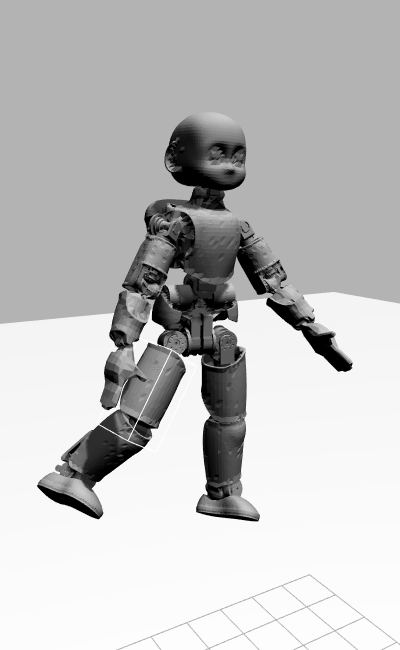
\includegraphics[width=0.23\textwidth]{images/contributions/chapter_8/astronaut_1.png}
    }
    \subfloat{
        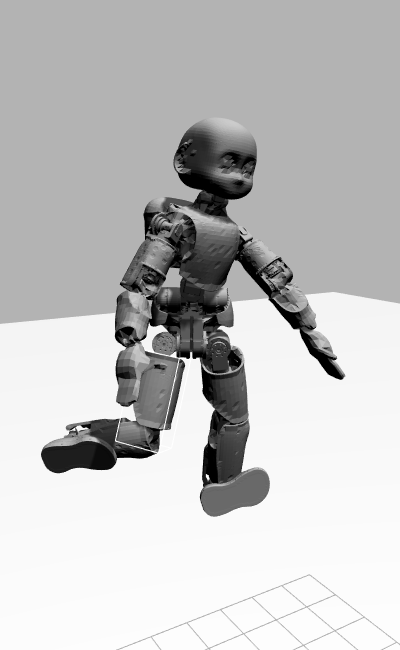
\includegraphics[width=0.23\textwidth]{images/contributions/chapter_8/astronaut_2.png}
    }
    \subfloat{
        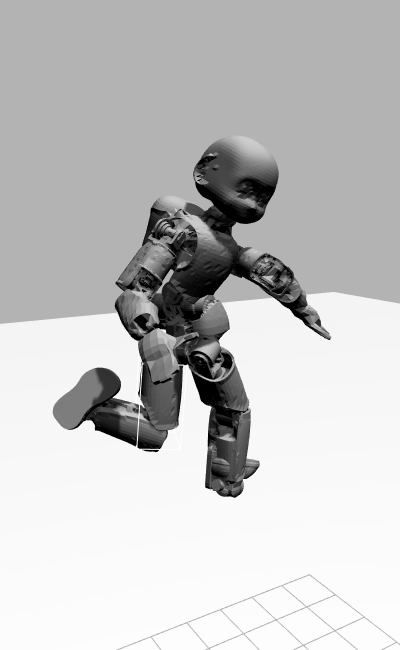
\includegraphics[width=0.23\textwidth]{images/contributions/chapter_8/astronaut_3.png}
    }
    \subfloat{
        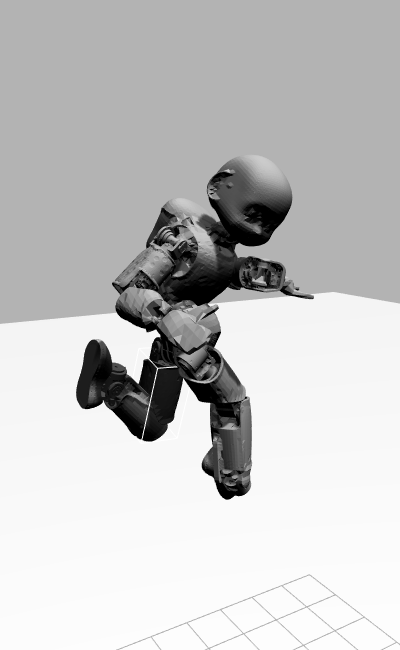
\includegraphics[width=0.23\textwidth]{images/contributions/chapter_8/astronaut_4.png}
    }
    \caption{Sequence showing four time instants of the astronaut simulation used for both the assessments of the momentum conservation and the energy conservation. In the former experiment, the joints are actuated with random torques, while in the latter, the joints are not actuated and evolve in open-loop accordingly to their initial velocity.}
    \label{fig:astronaut_experiment}
\end{figure}

In this section, we evaluate the simulation accuracy of \jaxsim through the astronaut simulation~\parencite{erezSimulationToolsModelbased2015s, howell_dojo_2022}, in which a robot model is simulated in a world without gravity.
The experiment is composed of two phases, both of which can be illustrated by Figure~\ref{fig:astronaut_experiment}.
In the first phase, the model is actuated for 1 second with random torques starting from a configuration with zero velocity and, therefore, zero momentum.
The simulation is performed with all lossy components (like joint friction) disabled, therefore, due to momentum conservation, the momentum should remain zero over the entire horizon.
In the second phase, the model evolves for 100 seconds without actuation from the configuration reached in the previous phase.
Also in this case, since there is no loss, the total mechanical energy of the system (\ie the sum of the kinetic and potential energies defined in Equation~\eqref{eq:kinetic_and_potential_energies}) should remain constant over the entire horizon due to energy conservation.

We perform this experiment using the model of the iCub robot with a configuration characterised by 23 of its \acp{DoF}.
The experiment is executed at different integration step sizes and with both the forward Euler and \ac{RK4} integrators.
We compare the results against Gazebo Sim running with its default DART physics engine.
The two simulators use the same model description of iCub.
The random actuation applied in the first phase is generated by sampling a torque for each joint from a uniform distribution $\tau \sim \mathcal{U}(-0.500, 0.500) \; Nm$.
The torques trajectory is generated offline at the lowest simulated frequency and up-sampled with zero-hold for higher frequencies.
In order to get a fair comparison between \jaxsim and Gazebo, we enable the optional 64-bit support of \jax.
The results of the momentum conservation and energy conservation experiments are shown, respectively, in Figure~\ref{fig:jaxsim_conservation_momentum} and Figure~\ref{fig:jaxsim_conservation_energy}.

In the results of the first phase, it can be seen that in almost all configurations the 6D momentum drifts from its initial value.
Particularly, all configurations show a more substantial drift in conjunction with larger integration steps.
The configuration of \jaxsim with the \ac{RK4} integrator can outperform the other ones, showing acceptable drifts with steps below $20$~ms.
Considering as acceptable a drift of $0.1$\% after $1$~s of simulation, also the forward Euler integration scheme stepping at $0.001$~s falls within this limit.

In the results of the second phase, a similar drift could be noticed in all the tested configurations.
Also in this case, \jaxsim with the \ac{RK4} integrator yields the lowest drift comparable to machine precision.
The results of Gazebo Sim and \jaxsim with forward Euler integrating with a step size of $0.001$~s are comparable, while Gazebo Sim performs better in the configuration with the larger $0.010$~s step.
The drift of \jaxsim with the larger integration step $0.010$~s and the \ac{RK4} integrator are comparable to the other configurations integrating with $0.001$~s steps, highlighting the benefits of higher-order integration schemes already discussed in Section~\ref{sec:integrators}.

An excessive increase of the integration step is generally not advisable also for reasons not strictly related to the integration accuracy.
In fact, the contact detection routine has no control over the stepping strategy, and excessively large steps could result in substantial instantaneous penetration depths that, depending on the selected terrain stiffness, could produce unrealistically big contact forces.

\begin{figure}
    \centering
    \resizebox{\textwidth}{!}{
    \includegraphics{images/contributions/chapter_8/jaxsim_conservation_momentum.tikz}}
    \caption{Momentum drift after 1 simulated second of the iCub humanoid robot in a world without gravity, starting from a configuration with zero velocity and applying random joint forces. The plot shows the norm of the linear and angular component of the momentum computed in inertial-fixed coordinates. Gazebo Sim failed to simulate the configuration with the $100$~ms step.}
    \label{fig:jaxsim_conservation_momentum}
\end{figure}

\begin{figure}
    \centering
    \resizebox{\textwidth}{!}{
    \includegraphics{images/contributions/chapter_8/jaxsim_conservation_energy.tikz}}
    \caption{Mechanical energy drift over 100 simulated seconds of the iCub humanoid robot in a world without gravity, starting from a configuration with a given generalized velocity.}
    \label{fig:jaxsim_conservation_energy}
\end{figure}

\subsubsection{Performance}

In this section, we evaluate the runtime performance of the \aclp{RBDA} implemented in \jaxsim against a state-of-the-art C++ implementation included in Pinocchio~\parencite{carpentier_pinocchio_2015, carpentier_pinocchio_2019}.

We compute the total time necessary to compute the output of the \ac{CRBA}, \ac{RNEA}, and \ac{ABA} algorithms.
To assess how much the execution time is affected by the topology of the simulated robot, we consider three different robot models with an increased number of \acp{DoF}.
In particular, we benchmark the 9~\acp{DoF} fixed-base Panda manipulator from Franka Emika, the 12~\acp{DoF} quadruped ANYmal C from ANYbotics, and the humanoid iCub from IIT.
Before running any test with \jaxsim, we call each algorithm one time so that it can get \ac{JIT} compiled since in this experiment we are interested in their runtime performance rather than compilation time.
For each bar in the plot, we first compute the mean time taken by a single run of 1000 executions of the algorithms, and then report the average over 10 of these runs.
Figure~\ref{fig:jaxsim_benchmark_algos} shows the resulting mean, where the variance of the 10 runs has been omitted since it's negligible for all algorithms.

The results are comparable for all three tested robot models.
The execution time of the \jaxsim algorithms compared to the implementation of Pinocchio are about 10 times higher when executed on \ac{CPU}, and 100 times higher when executed on \ac{GPU}.
These numbers are expected since Pinocchio algorithms are implemented entirely in \cpp and have been optimised for almost a decade.
Regardless, for all three robot models, the \jaxsim algorithms executed on \ac{CPU} do not exceed $250~\mu s$, making them compatible with a real-time loop running at a target rate of 1~kHz, in which a model-based controller might have to compute the mass matrix $M(\Qu)$ through \ac{CRBA} and the bias forces $h(\Qu, \Nu)$ through \ac{RNEA}.
Instead, the \ac{GPU} execution of a single instance of the algorithms exceeds 1~ms in most cases, making them incompatible with real-time usage.

\begin{figure}
    \centering
    \subfloat[]{
        \includegraphics[width=0.95\textwidth]{images/contributions/chapter_8/jaxsim_benchmark_algo_panda.tikz}
    }
    \\
    \subfloat[]{
        \includegraphics[width=0.95\textwidth]{images/contributions/chapter_8/jaxsim_benchmark_algo_anymal.tikz}
    }
    \\
    \subfloat[]{
        \includegraphics[width=0.95\textwidth]{images/contributions/chapter_8/jaxsim_benchmark_algo_icub.tikz}
    }
    \caption{Benchmark of the \acp{RBDA} implemented in \jaxsim against those implemented in Pinocchio. (a) shows the results of the 9-\acp{DoF} fixed-base Panda manipulator from Franka Emika, (b) the results of the 12-\acp{DoF} quadruped ANYmal~C from ANYbotics, and (c) the results of the 32-\acp{DoF} humanoid iCub from IIT. The execution of \jaxsim's algorithms run on average 10 times slower than Pinocchio when executed on \acs{CPU}, and 100 times when executed on \acs{GPU}.}
    \label{fig:jaxsim_benchmark_algos}
\end{figure}

\subsubsection{Scalability}

In the previous test, we assessed the performance of a single execution of the benchmarked algorithms implemented in \jaxsim.
The major strengths of \jaxsim appear when the characteristics of hardware accelerators are exploited, performing multiple executions in parallel.
In this test, we evaluate the scalability of \jaxsim by increasing the number of parallel instances exploiting the auto-vectorization capabilities of \jax.
Instead of testing parallel calls of the \acp{RBDA}, we consider a more practical scenario of a 1~ms simulation step with the forward Euler integration scheme.
We benchmark the performance on the 23~\acp{DoF} model of the iCub humanoid with 8 collidable points corresponding to the vertices of the two boxes that model its feet collision shapes.
We compute the \emph{equivalent} \ac{RTF} of the parallel integration, which consists of the ratio between the total simulated time and the time it took to compute it.
For example, if the parallel integration of 10 models takes 1~ms, the equivalent \ac{RTF} is 10.
A higher \ac{RTF} corresponds to a better sampling efficiency.
This test is performed on the same laptop as the previous tests, and also on a workstation with a more powerful \ac{GPU}, whose specifications are reported in Table~\ref{tab:specifications}.
For each point in the plot, we first compute the mean time of a single run over 100 integration steps, and then report the average over 10 of these runs.
The results of the \ac{CPU} and \ac{GPU} executions are shown in Figure~\ref{fig:jaxsim_benchmark_parallel}, where the variance of the 10 runs has been omitted since it is negligible for all executions.

On the laptop setup, the integration step on \ac{CPU} starts with a \ac{RTF} greater than 1 already with a single instance.
A single \ac{CPU} core is able to reach a \ac{RTF} of about 5 with 16 parallel models, showing some benefits of parallel integration also on this type of hardware.
With more than 16 models, increasing the number of models does not give any benefit to the equivalent \ac{RTF} as the execution time grows linearly with the number of models.
The integration step of \ac{GPU} starts with a lower \ac{RTF} of 0.11.
This effect is expected since a single \ac{GPU} core is typically less powerful than a \ac{CPU} core.
However, the parallel integration on \ac{GPU} is able to scale without showing any overhead until 128 models.
The equivalent \ac{RTF} on \ac{GPU} peaks at a value of about $19$ between 512 and 1024 parallel models.
On this hardware, the 512-1024 range is justified by the number of CUDA cores equal to 640.

A similar trend is observed regarding the workstation \ac{GPU}.
Although being more modern and powerful, the execution is slightly slower on this high-end \ac{GPU} compared to the laptop, starting from a \ac{RTF} of 0.08.
In this case, the \ac{GPU} has 4608 CUDA cores.
It can be noticed that the region in which the performance on \ac{GPU} scales horizontally without additional overhead is much larger, and start flattening in the range 4096-8192, which also in this case is close to the number of CUDA cores of the setup.
The peak \ac{RTF} of this high-end \ac{GPU} is about 200.

\begin{figure}
    \centering
    \resizebox{\textwidth}{!}{
        \includegraphics{images/contributions/chapter_8/jaxsim_benchmark_parallel.tikz}
    }
    \caption{Comparison of parallelization performance of a simulation step executed on \acs{CPU} and \acp{GPU}. The simulated models are 23~\acp{DoF} replicas of the iCub humanoid robot, and the simulation step length is $1~ms$ with a forward Euler scheme. The time taken by the \acs{CPU} scales mostly linearly with the number of simulated models, while the \acp{GPU} are able to exploit the parallel capability almost up to their CUDA cores (640 on the laptop, 4608 on the workstation). For each sample, we show the equivalent \acs{RTF}. The \ac{CPU} cannot scale well over the number of models when integrating more than 16 replicas. Instead, the \acp{GPU} show an interval that depends on their parallellization capabilities in which the execution time is not affected significantly by the number of integrated models. Also on \acp{GPU}, however, the performance start degrading when the number of integrated models exceeds the available CUDA cores.}
    \label{fig:jaxsim_benchmark_parallel}
\end{figure}

\newpage
\section{Validation}
\label{sec:jaxsim_validation}

In this section, we perform a validation of \jaxsim for generating synthetic data for robot learning.
We develop an environment exposing the \texttt{gym.Env} interface with \jaxsim, and show the sampling performance that can be reached by stepping a large number of parallel environments on a laptop \ac{GPU}.
We then plug the vectorized environment in a \ac{RL} pipeline for training a policy with the \ac{PPO} algorithm.
Finally, for presenting evidence that the data generated through the methods proposed in this thesis can be used in an out-of-distribution setting, we execute and evaluate the policy on a comparable dynamics simulated this time with Mujoco.

The out-of-distribution validation is also known in the literature as sim-to-sim~\parencite{salvato_crossing_2021, muratore_robot_2022, bellegarda_robust_2021, du_auto-tuned_2021}.
Given that one of the assumptions for an effective transfer is the availability of a robust policy trained in the original setting, we consider as target task to learn the swing-up of an underactuated cartpole.
This task is similar to the canonical benchmark of cartpole balancing~\parencite{brockman_openai_2016}, in which the pole starts from an almost balanced configuration and the actions space is discrete (selecting either a positive of negative constant force to apply to the cart).
This cartpole balancing, however, is excessively simple, and it is not really representative of the typical problems in robotics, usually characterised by continuous action spaces.
The swing-up task makes the policy learning much more difficult by starting the episodes with an arbitrary pole position (also pointing down).
This diversity makes a big difference since it requires the policy to be considerably long-sighted, to the extent to learn to perform some initial swing to build up momentum before attempting to perform a proper balancing.

All experiments presented in this section have been executed on a laptop whose specifications are reported in Table~\ref{tab:laptop_specifications_validation}.

\begin{table}
    \small
    \centering
    \begin{tblr}{
        colspec={Q[c, m]Q[c, m]},
        row{even} = {bg=gray9},
        row{1} = {font=\bfseries\footnotesize},
    }
        \toprule
        Specification & Value \\
        \midrule
        Intel CPU & i7-10750H \\
        Nvidia GPU & GeForce GTX 1650 Ti Mobile \\
        CUDA cores & 1024 \\
        Operating system & Ubuntu 22.04 \\
        Nvidia driver & 530.41.03 \\
        CUDA & 11.2.2 \\
        cuDNN & 8.8.0.121 \\
        \jax & 0.3.15 \\
        Mujoco & 2.3.5 \\
        \bottomrule
    \end{tblr}
    \caption{Specifications of the machine used to execute the validation experiments.}
    \label{tab:laptop_specifications_validation}
\end{table}

\subsection{Sampling Experience for Robot Learning}

The cartpole is a fixed-base model composed by a pole (shaped as a long and thin cylinder) connected through an un-actuated revolute joint to a cart (shaped as a box).
The cart can move along a track, whose displacement is simulated as a prismatic joint.
The linear force corresponding to this prismatic joint is the control input of the system.
Figure~\ref{fig:cartpole_swingup} reports a visualisation of the cartpole model.

\begin{figure}
    \centering
    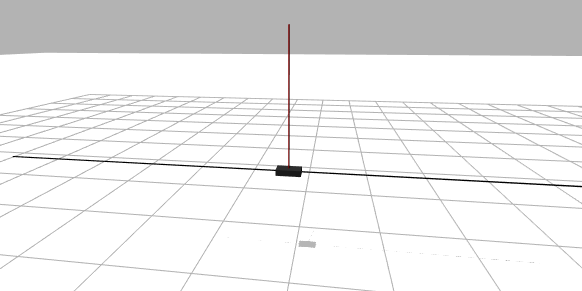
\includegraphics[width=0.85\textwidth]{images/contributions/chapter_8/cartpole.png}
    \caption{Illustration of the cartpole model in the $\theta = d = 0$ configuration.}
    \label{fig:cartpole_swingup}
\end{figure}

\begin{table}
    \small
    \centering
    \begin{tblr}{
        colspec={Q[c, m]Q[c, m]},
        row{even} = {bg=gray9},
        row{1} = {font=\bfseries\footnotesize},
    }
        \toprule
        Property & Value \\
        \midrule
        Integrator & Semi-implicit Euler \\
        Integrator step & $0.0005\,$~s \\
        Environment step & $0.050\,$~s \\
        Control frequency & $20\,$Hz \\
        Action dimension & 1 \\
        Observation dimension & 4 \\
        Action space & $[-50,\, 50]\,$~N \\
        {Maximum episode steps} & $200$ \\
        Parallel environments & $512$ \\
        Equivalent \ac{RTF} & $24.38$ \\
        \bottomrule
    \end{tblr}
    \caption{Properties of the environment implementing the cartpole swing-up task.}
    \label{tab:environment_properties_cartpole}
\end{table}

\begin{table}
    \small
    \centering
    \begin{tblr}{
        colspec={Q[c, m]Q[c, m]},
        row{even} = {bg=gray9},
        row{1} = {font=\bfseries\footnotesize},
    }
        \toprule
        Parameter & Value \\
        \midrule
        Discount rate $\gamma$ & $0.95$ \\
        Clip parameter $\epsilon$ & $0.1$ \\
        Target \acs{KL} divergence & $0.025$ \\
        Learning rate $\alpha$ & $0.0003$ \\
        \acs{GAE} parameter $\lambda$ & $0.9$ \\
        Batch size & $2560$ \\
        Minibatch size & $256$ \\
        Number of \small{SGD} epochs & $10$ \\
        \bottomrule
    \end{tblr}
    \caption{PPO parameters for the the cartpole swing-up environment.}
    \label{tab:ppo_parameters_cartpole}
\end{table}

\begin{description}
%
\item[Observation]
The observation of the system is composed of the position and velocity of both joints.
If $\theta \in [-\pi,\, \pi]\,$rad is the angle of the un-actuated revolute joint (where $\theta = 0$ is a balanced pole), $d \in [-2.5,\, 2.5]\,$m the displacement of the prismatic joint, and $\omega = \dot{\theta}$ the pole velocity, we can define the observation as $\mathbf{o} = ( d, \dot{d}, \theta, \omega) \in \realn^4$.
%
\item[Action]
The action of the system is the linear force $a = f \in [-50,\, 50]\,\text{N}$ corresponding to the joint moving the cart.
It's worth noting that the action is continuous and its magnitude is not large enough to accelerate the cart and bring the pole in vertical position without swinging first.
%
\item[Environment details]
The environment simulates the physics with \jaxsim.
We use a semi-implicit Euler integrator with a step of $500\,\mu$s.
After the agent sets an action through the exposed \texttt{gym.Env} interface, we step the environment for $0.050\,$s, therefore performing $100$ physics steps each time.
The resulting control frequency, that is the update rate at which the policy applies its actions, results equal to $20\,$Hz.
The environment is implemented as a continuous control task with termination only occurring if the observation is outside its space.
In absence of termination, episodes are truncated after $200$ steps.
All environment properties are reported in Table~\ref{tab:environment_properties_cartpole}.
%
\item[Reward]
The reward function used to learn the swing-up task is the following:
%
\begin{align*}
    &r_t(s_t, a_t, s_{t+1}) = \\
    &\quad r_{\text{alive}} + r_{\text{balance}} - 0.001 \, c_{\text{action}} - 0.1 \, c_{\text{vel}} - 0.5 \, c_{\text{displacement}}
    ,
\end{align*}
%
where $r_{\text{alive}}$ is set to $1.0$ when the environment is not terminal and $0$ otherwise, $r_{\text{balance}} = \cos{\theta}$ rewards the pole to be in a balanced state (characterised by $\theta=0)$, $c_{\text{action}} = \lVert \tau \rVert$ penalises large actuated forces, $c_{\text{vel}} = \lVert \Shaped \rVert$ penalises large joint velocities, and $c_{\text{displacement}} = \abs{d}$ penalises the cart to be far from the middle point of the track.
%
\item[Agent Networks]
We want to train a policy with \ac{RL} capable of bringing the pole to a balancing position from any state belonging to the observation space, and maintain the balance as long as possible.
The agent is composed of two neural networks corresponding to the actor --the policy-- and the critic --the return--, having two hidden layers with $512$ neurons each with {\small ReLU} activation function.
The input layer of both networks has a size of $4$ (the observation dimension).
The critic network has an output layer with just one dimension corresponding to the return, correctly bootstrapped from the value function is case of episode truncation.
The actor network encodes a univariate Gaussian distribution (the environment action is a scalar), therefore it has one output corresponding to the distribution mean and has a free parameter part of the optimisation parameters corresponding to the logarithm of the distribution's variance.
The variance is initialised with the value of $\log \sigma = \log(0.05)$.
The neural networks are optimised with Adam~\parencite{kingma_adam_2017} using a learning rate $\alpha = 0.0003$.
%
\item[Algorithm]
For the same reasons explained in Chapter~\ref{ch:learning_from_scratch}, we train the policy with the \ac{PPO} algorithm introduced in Section~\ref{sec:ppo}, configured with the clip parameter $\epsilon=0.1$.
We estimate the return from the advantage computed with \ac{GAE}, introduced in Section~\ref{sec:gae} as $R_t = \hat{A}^\text{GAE}_t + V_t$, configured with $\lambda=0.9$ and a discount rate $\gamma = 0.95$.
We use the \ac{PPO} implementation of \texttt{stable-baselines3}~\parencite{raffin_stable-baselines3_2021} that, instead of using a \ac{KL} penalty, stops the training epochs when the approximated \ac{KL} divergence exceeds a given value.
All the \ac{PPO} parameters are reported in Table~\ref{tab:ppo_parameters_cartpole}.
%
\item[Sampling]
We optimise the policy by acquiring five samples from $512$ parallelised environments running on \ac{GPU}, resulting to an equivalent \ac{RTF} of about $25$ on the machine used to run the experiments.
The number of environments has been selected by choosing the best equivalent \ac{RTF} of the \ac{JIT}-compiled vectorized \texttt{gym.Env.step} through a grid-search in the $N_\text{envs} = 2^p,\, p \in \{1,\, 2,\, 3,\, \dots, 12\}$ range.
The collected batch of trajectories, containing a total of $2560$ samples and equivalent to about 2 minutes of experience, is then split in $10$ minibatches of $256$ samples.
We perform $10$ optimisation epochs on the same batch of trajectories, that can be interrupted earlier in case the approximated \ac{KL} divergence \wrt the distribution corresponding to the previous policy exceeds $0.025$.
Before optimising the \acp{NN} of the agent, the collected observations and rewards are normalized by computing a running mean and standard variance.
Finally, in order to obtain a more robust policy, we inject some Gaussian noise with zero mean and $\sigma=0.05$ to the actions before being applied to the environment.
%
\end{description}

\begin{figure}
    \centering
    \resizebox{0.75\textwidth}{!}{
    \includegraphics{images/contributions/chapter_8/learning_curves.tikz}}
    \caption{Learning curves of the cartpole swing-up task. The plot reports the mean and standard deviation of the average rewards $\hat{r}_t^{(k)}$ computed over $k=10$ different training executions. For each individual training, the average reward $\hat{r}_t$ in the considered parallel setting is computed by averaging at each time step the $512$ rewards received from the vectorized \texttt{gym.Env.step}.}
    \label{fig:learning_curve_cartpole_swingup}
\end{figure}

\newpage
Figure~\ref{fig:learning_curve_cartpole_swingup} shows the learning curve of 10 trainings initialised with different seeds.
The policy is able to learn effective swing-up and balancing behaviours in $500000$ steps, corresponding to about $7$ hours of equivalent experience.
On the machine used to run this experiment, each training runs for approximately $15$ minutes.
The reward grows mostly monotonically with a limited variance, showing that the chosen parameters ensure stable policy updates, preventing optimisation steps too large that would destroy the previously obtained performance.

\subsection{Sim-to-sim Policy Transfer}

\begin{table}
    \small
    \centering
    \begin{tblr}{
        colspec={Q[c, m]Q[c, m]},
        row{even} = {bg=gray9},
        row{1} = {font=\bfseries\footnotesize},
    }
        \toprule
        Property & Value \\
        \midrule
        \texttt{timestep} & $0.001$ \\
        \texttt{integrator} & \texttt{RK4} \\
        \texttt{solver} & \texttt{Newton} \\
        \texttt{iterations} & $100$ \\
        \texttt{contype} & $0$ \\
        \bottomrule
    \end{tblr}
    \caption{Mujoco properties used for the sim-to-sim evaluation of the trained cartpole swing-up policy. Refer to the official documentation at \url{https://mujoco.readthedocs.io} for a detailed explanation of the options.}
    \label{tab:mujoco_parameters}
\end{table}

In this section, we attempt to evaluate the trained policy in an out-of-distribution setting.
This setting could represent any environment that differs from the one where the policy has been trained.
It serves as evidence that it's possible to deploy a policy obtained from training over synthetic data generated efficiently by a parallel simulator into an equivalent environment running on a different runtime.
In particular, this experiment can be seen as a sim-to-sim policy transfer.

Similarly to Section~\ref{sec:sliding_box_inclined_plane}, we use the Mujoco simulator as out-of-distribution setting.
We translated the \ac{URDF} of the cartpole model loaded in \jaxsim in the training environment to an equivalent \ac{MJCF} that can be imported in Mujoco.
Then, we included in the same file the configuration of the physics engine, whose parameters are reported in Table~\ref{tab:mujoco_parameters}.
The chosen parameters expose a simulation characterised by the same control rate ($20\,$Hz), but in this case the physics is simulated in a different simulator using an integrator of a different family and different constraint solver.

The Mujoco environment is only used for producing the state-action trajectory $\tau$ from a given initial observation $\mathbf{o}_0$, where the action is obtained by performing inference of the trained policy.
In order to perform a proper exploitation of the policy, we sample deterministically by taking the inferred mean of the Gaussian distribution described by the policy, \ie $a_t = \mu_{\boldsymbol{\theta}}(\mathbf{o}_t)$.

The first evaluation we perform in this setting is a comparison between the swing-up trajectory obtained by running the policy in the training environment simulated with \jaxsim and the out-of-distribution environment simulated with Mujoco.
In order to obtain a meaningful comparison, we consider as initial observation the cart resting in the center of its track and the pole pointing down, both with zero velocity, \ie $\mathbf{o}_0 = (0, 0, \pi, 0)$.
The two trajectories are shown in Figure~\ref{fig:cartpole_trajectory_jaxsim_vs_mujoco}, where it can be noticed that the policy performance are comparable in both simulators.
The policy is able to succeed in the swing-up task and the resulting trajectories in both simulators are almost identical.

As second evaluation, starting from the same initial observation $\mathbf{o}_0$ considered in the first evaluation, we assess the policy swing-up performance on different variations of the cartpole environment simulated with the out-of-distribution Mujoco.
In particular, we modify some physical parameters and evaluate whether the learned policy is robust enough to succeed in the task.
In the first variation, we double the mass of both the cart and the pole, taking care to compute the new $3\times 3$ inertia matrices corresponding to the primitive shape of the bodies.
In the second variation, in addition to the increased masses, we include joint damping, \ie a frictional force proportional to the joint velocity that opposes the motion direction.
For a revolute joint, its contribution is $\tau_\text{damping} = - k_v \dot{\theta}$.
Figure~\ref{fig:cartpole_mujoco_change_parameters} reports the curves simulated in the out-of-distribution Mujoco simulator using out-of-distribution model parameters.
Despite the out-of-distribution environment, it can be seen that the policy learned in a highly parallel setting simulated with \jaxsim on \ac{GPU} succeeds in swing-up task.
As it can be expected, the performance are affected by the change of parameters.
For example, the policy is able to reach the balancing state by using only one swing in the setting with nominal parameters.
Instead, in the two variations, the policy needs two swings.

It's worth noting that the policy has been trained only using the nominal parameters.
Often, in order to obtain more robust policies, the inertial parameters of the simulated model become part of domain randomization.
In our case, we did not randomize any parameter.

\begin{figure}
    \centering
    \resizebox{0.99\textwidth}{!}{
    \includegraphics{images/contributions/chapter_8/cartpole_jaxsim_vs_mujoco}
    }
    \caption{Sim-to-sim comparison of the trajectories obtained by exploiting the swing-up policy learned in a \jaxsim environment. The \jaxsim curves correspond to an in-distribution setting, where the policy is evaluated in the same simulator that generated training data. Instead, the Mujoco curves correspond to an out-of-distribution setting, where the policy is evaluate in a simulator different from the one that generated training data. Note that $\theta$, due to its range, is projected in the $[-\pi,\, \pi]$ range.}
    \label{fig:cartpole_trajectory_jaxsim_vs_mujoco}
\end{figure}

\begin{figure}
    \centering
    \resizebox{0.99\textwidth}{!}{
    \includegraphics{images/contributions/chapter_8/cartpole_benchmark_mujoco}
    }
    \caption{Trajectories of the cartpole swing-up policy acting on the out-of-distribution environment simulated in Mujoco. The \emph{nominal} curves are obtained by running the policy on a cartpole model having nominal masses of both the cart and the pole, and with no joint damping. The \emph{mass} curves show the obtained trajectories with the model having the masses of both bodies multiplied by $2x$. The \emph{mass+damping} curves are generated in a setting that extends the \emph{mass} one by also considering for both joints a damping with $k_v=0.015$. Note that in this case, we removed the bounds of the pole angle, showing more clearly the number of swings used by the policy to reach the balancing state.}
    \label{fig:cartpole_mujoco_change_parameters}
\end{figure}

\section{Conclusions}

In this chapter, we proposed \jaxsim, a new physics engine capable of executing multibody simulations on modern hardware accelerators.
\jaxsim simulates the dynamics of free-floating mechanical systems through a reduced coordinates approach, therefore guaranteeing that joint constraints are never violated.
Regarding the interaction with the environment, it is currently capable of detecting collisions between a smooth ground surface not necessarily planar and points belonging to the collision shapes of the links.
Being implemented in reduced coordinates, it allows to efficiently compute all terms of the \ac{EoM} that are fundamental for model-based control at any simulated step.
We have validated its integration accuracy, obtaining either comparable or better results than Gazebo Sim, depending on the adopted integration scheme.
We also benchmarked the \acp{RBDA} performance, finding that \ac{JIT}-compiled Python code on \ac{CPU} runs 10 times slower compared to a state-of-the-art \cpp implementation, remaining in any case compatible with real-time usage.
Nonetheless, the best characteristics of \jaxsim emerge when modern hardware accelerators are exploited in highly parallel computations.
We have shown that it can reach a \ac{RTF} of 20 on a laptop and 200 on a workstation.
Applications requiring sampling experience with high throughput such as those characterising \ac{RL} research, would benefit the most from these performances.
Furthermore, generating physics data directly in the same device where function approximators are optimised would remove any overhead related to the data transfer from the \ac{CPU}.
We intend to investigate these directions in future activities.
Finally, we trained a policy to solve a continuous control problem simulated with \jaxsim, providing details on the parallelization level that can be reached for sampling synthetic data in a characteristic robot learning application.
Then, to provide evidence that it's possible to deploy policies obtained from training by sampling from highly parallel simulators, we performed a sim-to-sim transfer and evaluated the policy performance on a out-of-distribution simulator and physical parameters.
The obtained \ac{RL} setting is much simpler compared to one adopted in Chapter~\ref{ch:learning_from_scratch}.
The possibility to parallelize sampling on hardware accelerators removes the need to rely on distributed settings running on a cluster of machines, that is difficult to create, maintain, and handle.
A single-process application can deploy both sampling and \acp{NN} on the same \ac{GPU}, with no overhead related to network transport.
Beyond being easier to deploy in a {\small HPC} setting, this approach may lead to a faster development and prototyping.

\jaxsim still presents multiple limitations in this first version.
Firstly, the shown performance were obtained in a setting where no exteroception was necessary.
Integrating basic rendering functionality would surely negatively affect them.
Furthermore, collisions between links are not yet supported, limiting the adoption for robot manipulation.
Finally, it does not yet allow enforcing additional dynamic constraints like joint limits, and closed kinematic chains.
To conclude, although the automatic differentiation capability provided by the \jax framework has not yet been thoroughly tested with the \jaxsim algorithms, its combination with the smooth dynamics given by the contact-aware state-space representation opens up exciting research directions that will be explored in the future.
